\documentclass{myhw}
\usepackage{ctex}
\linespread{1.05}        % Palatino needs more leading (space between lines)
\usepackage{extarrows}
\usepackage{mathrsfs}
\usepackage{braket}
\usepackage{enumerate}
\titleformat{\section}[runin]{\sffamily\bfseries}{}{}{}[]
\titleformat{\subsection}[runin]{\sffamily\bfseries}{}{}{}[]
\renewcommand{\exname}{Exercise }
\renewcommand{\subexcounter}{(\alph{homeworkSectionCounter})}
\newcommand{\id}{\text{Id}}
\newcommand{\tr}{\text{Tr}}
\newcommand{\rib}{\text{Rib}}

\title{Design and Analysis of Algorithms}

\begin{document}
\begin{center}
\noindent{\Large \heiti 2020年算法设计与分析 \textbf{Assignment-1}}

\vspace{0.5cm}

Due: OCT 19, 2020

\vspace{0.5cm}
\noindent {\large 郭宇航  202021080728}
\end{center}
\begin{homeworkProblem}
求解下列递归式的渐进解:
\[
\begin{split}
&(1)\quad f(n)=9f(n/6)+n\log n\\
&(2)\quad f(n)=2f(n-3)+n\\
&(3)\quad f(n)=4f(n/2)+n^2
\end{split}
\]

\end{homeworkProblem}
\begin{solution}
(1) 由于$f(n)=n\log n$,因为无法直接使用简单的master theorem求解。但是我们可以使用主定理对其进行分析。首先不难得到$a=9,b=6$. 那么$n^{\log_b a}=n^{\log_6 9}$, 同时$f(n)=n\log n$. 
\[
\frac{n^{\log_6 9}}{n\log n}=\frac{n^{(\log_6 9) -1}}{\log n}=\frac{n^{\log_6 \frac{3}{2}}}{\log n}
\]
由于分子是一个多项式时间复杂度,分母是一个对数时间复杂度,所以我们可以认为$f(n)$是要多项式地小于$n^{\log_b a}$的,也就是说我们能够找到一个$\epsilon >0$使得$f(n)=O(n^{\log_b (a-epsilon)})$. 因此我们可以得到:
\[
T(n)=\Theta(n^{\log_6 9})
\]
\end{solution}
\begin{solution}
(2) 由于$f(n)=2f(n-3)+n$的形式不能够满足$b>1$的情况,因此这个问题无法使用master theorem处理。这里考虑使用递归树的方式处理,考虑这个递推关系式,对于原规模为$n$的问题,可以分解为两个规模为$n-3$的子问题,层层递归下去,我们不难发现这个递归树一共会有$n/3$层,同时每一层进行的运算为$n,n-3,n-6,\cdots$. 从而总运算数可以表示为一个等差数列的和:
\[
T(n)=\frac{n+1}{2}\times \frac{n}{3}=\frac{n^2+n}{6}
\]
从而问题的结果为:$T(n)=\Theta(n^2)$.
\end{solution}

\begin{solution}
(3) 这个问题可以直接使用master theorem进行求解:$a=4,b=2,c=2$.
得到$c=2=\log_b a=\log_2 4=2$.
因此这个问题的结果为:$T(n)=\Theta(n^2\log n)$.
\end{solution}
\begin{homeworkProblem}
将下列6个函数按照渐近增长率由低到高进行排序,要求写出判断依据。
\[
\begin{split}
&f_1(n)=\sqrt{n}+(\log n)^n,\quad f_2(n)=2^{\log n +\log \log n},\quad f_3(n)=\log\left(n^{100}\times 3^n\right)\\
& f_4(n)=n^{200}+3^{n},\quad f_5(n)=\log n^{100\log n},\quad f_6(n)100^n+n!\\
&(\text{各log函数的底数都为}2)
\end{split}
\]
\end{homeworkProblem}
\begin{solution}
首先对6个函数进行化简:
\begin{itemize}
\item $f_1(n)=\sqrt{n}+(\log n)^{100}$ 多项式时间
\item $f_2(n)=2^{\log n+\log \log n}=n\log n$.
\item $f_3(n)=\log (n^{100}\times 3^n)=100\log n+n\log 3$ 多项式时间
\item $f_4(n)=n^{200}+3^n$ 指数时间
\item $f_5(n)=\log n ^{100\log n}=100 \log n \log n$
\item $f_6(n)=100^n+n!$ 阶乘时间
\end{itemize}
经过化简之后可以很容易地得到关于这6个函数渐近增长率由低到高的排序:
\[
f_5(n)<f_1(n)<f_3(n)<f_2(n)<f_4(n)<f_6(n)
\]
\end{solution}
\begin{homeworkProblem}
平面上有$N\times M$个格子,每个格子中放着一定数量的苹果。从左上角的格子开始,每一步只能向下走或是向右走,每次走到一个格子上就把格子里的苹果收集起来,这样最终最多能收集到多少个苹果。设计算法求解上述问题,给出算法的伪代码描述即可。
\end{homeworkProblem}
\begin{solution}
使用简单的动态规划算法。
\end{solution}
\begin{homeworkProblem}
计算下图中从$S$到$T$的最大流,并给出最小割。
\begin{figure}[!htbp]
\centering
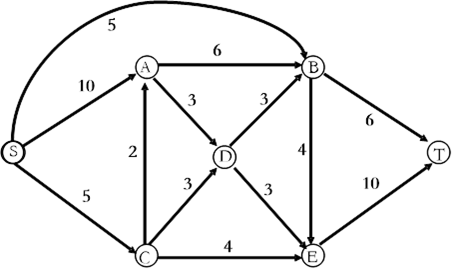
\includegraphics{fig5.png}
\end{figure}
\end{homeworkProblem}
\end{document}
